\documentclass{article}
\usepackage{tikz}
\usetikzlibrary{shapes,arrows}
\usepackage{pdflscape}
\usepackage[papersize={10.5cm, 3.5cm}, text={10.5cm, 3.6cm}]{geometry}
\usetikzlibrary{decorations.text}
\usepackage{xcolor}
% \selectcolormodel{gray}

% What do people speak in Czech_Republic ?

\begin{document}
\thispagestyle{empty}
%\begin{landscape}
\begin{center}
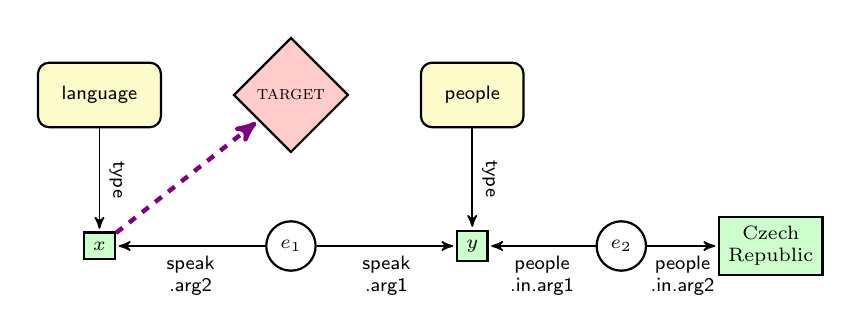
\begin{tikzpicture}[
  font=\sffamily,
  every matrix/.style={ampersand replacement=\&,column sep=0.9cm,row
sep=0.8cm,font=\scriptsize},
  entity/.style={draw,thick,rectangle,fill=green!20},
  word/.style={draw,thick,ellipse,fill=blue!20,},
  mediator/.style={draw,thick,circle},
  entityType/.style={draw,thick,rounded corners,fill=yellow!20,inner
sep=.3cm,font=\sffamily\scriptsize},
  mathType/.style={draw,thick,diamond,fill=red!20},
  mediatorToEntity/.style={->,>=stealth',shorten
>=1pt,semithick,black,sloped,above,font=\sffamily\scriptsize},
  typeToEntity/.style={->,>=stealth',shorten
>=1pt,semithick,black,sloped,above,font=\sffamily\scriptsize},
  wordToEntity/.style={-,>=stealth',shorten >=1pt,ultra
thick,dotted,blue,sloped,above,font=\sffamily\scriptsize},
  entityToMath/.style={->,>=stealth',shorten >=1pt,ultra
thick,dashed,violet,sloped,above,font=\sffamily\scriptsize},
  collapseEdge/.style={-,>=stealth',shorten >=1pt,ultra
thick,dashed,sloped,above,font=\sffamily\scshape,bend right=20},
  every node/.style={align=center}]

  % Position the nodes using a matrix layout
  \matrix{
    \node[entityType] (tLanguage) {language}; \& \node[mathType] (mLanguage) {\textsc{target}}; \& \node[entityType] (tPeople) {people}; \\
    
    \node[entity] (eLanguage) {$x$}; \& \node[mediator] (e1) {$e_1$}; \& \node[entity] (ePeople) {$y$}; \& \node[mediator] (e2) {$e_2$}; \& \node[entity] (eCzech) {Czech\\Republic}; \\
  };
 
  % mediator to entities
  \draw [mediatorToEntity] (e1) edge node[below] {speak\\.arg2}  (eLanguage);
  \draw [mediatorToEntity] (e1) edge node[below] {speak\\.arg1} (ePeople);
  
  \draw [mediatorToEntity] (e2) edge node[below] {people\\.in.arg1}  (ePeople);
  \draw [mediatorToEntity] (e2) edge node[below] {people\\.in.arg2} (eCzech);
  
  % types to entities
  \draw [typeToEntity] (tLanguage) edge node {type}  (eLanguage);
  \draw [typeToEntity] (tPeople) edge node {type}  (ePeople);
  
  % math types
  \draw [entityToMath] (eLanguage) edge node {}  (mLanguage);
\end{tikzpicture}
\end{center}

\end{document}